%% LyX 2.3.2 created this file.  For more info, see http://www.lyx.org/.
%% Do not edit unless you really know what you are doing.
\documentclass[english]{article}
\usepackage[T1]{fontenc}
\usepackage[latin9]{inputenc}
\usepackage{geometry}
\geometry{verbose}
\usepackage{babel}
\usepackage{array}
\usepackage{float}
\usepackage{graphicx}
\usepackage[unicode=true,pdfusetitle,
 bookmarks=true,bookmarksnumbered=false,bookmarksopen=false,
 breaklinks=false,pdfborder={0 0 0},pdfborderstyle={},backref=false,colorlinks=false]
 {hyperref}

\makeatletter

%%%%%%%%%%%%%%%%%%%%%%%%%%%%%% LyX specific LaTeX commands.
%% Because html converters don't know tabularnewline
\providecommand{\tabularnewline}{\\}

\makeatother

\begin{document}
\title{Thoughts on Nematic Order in Embryonic Morphogenesis}
\author{Laurent MacKay}
\maketitle

\section{Causes of apparent nematic order in living tissue}

Nematic order arises from neighbour-neighbour interactions between
rigid rod-like particles, producing long range orientational order.
In \cite{Kemkemer2000}, a mean-field approach is used to derive a
distortional energy for a cellular orientation field that is equivalent
to the classical free energy appearing nematic hydrodynamics equations.

\paragraph{Evidence}
\begin{enumerate}
\item In cultures of elongated cells, neighbour-neighbour interactions are
to be expected and indeed there is often long-range orientational
order in such cultures:
\begin{itemize}
\item Densely-packed neural progenitor cells in \cite{Kawaguchi2017} have
a degree of orientational order, which persists on the order of 10
cell lengths. Based on their observations at low densities, it seems
likely that the interaction is primarily mechanical (e.g., through
hydrostatic pressure).
\begin{itemize}
\item Similar cultures of NIH 3T3 cells show exquisite nematic ordering
\cite{Duclos2016}, where the steady-state position of +1/2 defects
in circularly confined domains is very well predicted by passive nematic
theory.
\end{itemize}
\item Loosely-packed melanocytes interact, primarily biochemically via their
dendrites, to produce a high degree of orientational order \cite{Gruler1999}.
\end{itemize}
\end{enumerate}

\paragraph{Complication}
\begin{enumerate}
\item However, unlike in nematic phases of actual liquid crystals, cells
can change shape quite drastically and will almost certainly do so
when dividing.
\begin{itemize}
\item Changes in density due to cell division have been suggested to enchance
(reduce) topological defects in extensile (contractile) models of
active nematics \cite{Doostmohammadi2015}.
\end{itemize}
\item Even within the same culture there may be regions where cells are
significantly more elongated than others (e.g., center vs. tips of
the ``plus''-shaped culture in Fig. 4a in \cite{Saw2017}).
\begin{enumerate}
\item I currently do not know how we could account for this variable cell
shape within the framework of nematic hydrodynamics, but its possible
that there is a way to do it. (Ask Jimmy about this).
\begin{enumerate}
\item An interesting microscopic/Hamiltonian-based model can be found in
\cite{Pai2016}.
\end{enumerate}
\begin{itemize}
\item The formalism in \cite{Kemkemer2000} would be also be good place
to start for deriving one.
\end{itemize}
\end{enumerate}
\end{enumerate}

\section{Effects of Nematic Order}

Assuming that nematic hydrodynamics are indeed at play during tissue
morphogenesis, what can be expected as a meaningful outcome of such
nematic order for a developping organism? Two ideas come to mind:
\begin{enumerate}
\item Orientational order can guide the flow of cells. If a topological
defect can be positioned consistently within an embryo, this may be
a way for the organism to organise its tissue (e.g., hydra).
\item Accumulation of cells at topolgical defects due to local differences
in stress/velocity.
\end{enumerate}

\subsection{Suggestive Experimental Results}

Below is a non-exhaustive list of experimental studies that show some
evidence for the biological-relevance of topological defects.

\begin{table}[H]
\begin{tabular}{|c|>{\centering}p{3cm}|c|>{\centering}p{3cm}|>{\centering}p{6cm}|}
\hline 
Defect & Biological Effect & Source & Cell-Type & Note\tabularnewline
\hline 
\hline 
+1/2 (-1/2) & increasing (decreasing) density & \cite{Kawaguchi2017} & NPC & unclear what the biological relevance is\tabularnewline
\hline 
+1/2 (-1/2) & new layer (hole) formation & \cite{Copenhagen2020} & Myxococcus xanthus (Soil Bacteria) & \tabularnewline
\hline 
+1/2 & apoptotic extrusion & \cite{Saw2017} & MDCK & See \ref{subsec:Critical-analysis-of}\tabularnewline
\hline 
+1 & development of cellular mounds & \cite{Guillamat2020} & C2C12 myoblasts & proposed to be reminscent of myotubule formation which C2C12 cells
are capable of forming\tabularnewline
\hline 
+1 & formation of an oriented ``cluster'' of cells & \cite{Kemkemer2000} & Migrating granulocytes surrounding immobile monocytes & Spontaneously occurs at low cell density when extracellular Ca2+ is
lowered\tabularnewline
\hline 
\end{tabular}\caption{}
\end{table}


\subsection{Critical analysis of the link between +1/2 defects and apoptotic
extrusion \label{subsec:Critical-analysis-of}}

In Saw2017, it is suggested that apoptotic extrusion is induced by
the high compressive stresses that develop at the heads of +1/2 topological
defects in monocultures of MDCK cells. While their quantitative analysis
is very convincing at establishing a correlation between high compressive
stress and apoptotic extrusion, I have two major issues with the line
of reasoning that leads them to draw a causal link.
\begin{enumerate}
\item Use of caspase-3 as a marker for apoptosis.
\begin{itemize}
\item Caspase-3 acts as an executioner, shredding the cytoskeleton to allow
for extrusion following loss of mechanical integrity. This causes
the cell to be pushed out of the plane by its neighbours (see \cite{Miroshnikova2017}
for a similar situation with less deadly results). Caspase-3 activation
occurs around 2-8 hours (typically 5+ hours) after the mechanical
induction of apoptosis \cite{Maeno2006,Lee2010}, while other caspase-independent
pathways activate in tens of minutes \cite{Pelling2009}.
\item Thus, caspase-3 seems a poor choice of marker for tracking apoptotic
cells prior to extrusion.
\item Given the flow of the monolayer (see Fig. \ref{fig:nematic_flow_and_extrusion})
and the timescale of the experiments, it seems likely that apoptosis
can be initiated far from the +1/2 defect.
\end{itemize}
\item A closer analysis of stress field and cellular movements do not support
a causal relationship.
\begin{itemize}
\item The data shown in Fig. 3b, Extended Data Fig. 1i, and Extended Data
Fig. 3e suggest correlations between compressive forces and extrusion.
N.B. that Extended Data Fig. 3e clearly shows that extrusion is not
limited to regions of compressive forces, the way the data is presented
in Fig. 3b obscures such facts.
\item By performing visual cell tracking on the supplemental movies, the
causal link starts to fall apart.
\item The region with high compressive forces slowly grows in size over
time (see green lines in Fig. \ref{fig:nematic_flow_and_extrusion}),
but it seems that the extruded cell only enters this region just prior
to extrusion (see note 1 in this subsection). Also, why do none of
the other cells in this region get extruded?
\end{itemize}
\begin{figure}[H]
\centerline{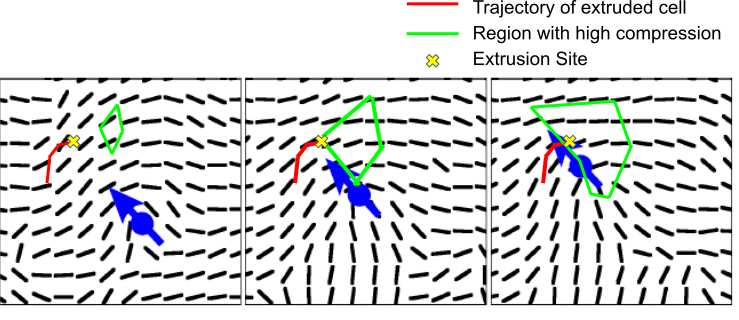
\includegraphics[width=14cm]{cell_and_defect_flow}}

\caption{Motion of an extruded cell (red line) and a +1/2 topological defect
(blue symbols), with extrusion (yellow symbol) occuring roughly where
the two trajectories meet. Note that the region of the culture which
develops high compressive forces (green lines) over time barely overlaps
with the cell's trajectory. Panels from left to right are taken at
160, 30, and 0 min prior to extrusion, respectively. Adapted from
\cite{Saw2017} by visual comparion of Fig. 1d and Supplemental Movie
4. \label{fig:nematic_flow_and_extrusion}}
\end{figure}

\item The proposed biological mechanism was not shown to actually be occuring
in their cultures (i.e., compression > YAP in cytoplasm > caspase-3
activation > extrusion).
\begin{itemize}
\item If YAP sequestering in the cytoplasm is indeed the causal link between
compressive forces and apoptosis, why did they never try to directly
correlate YAP distribution with compressive forces experienced by
a cell? Even better, force-history of the individual cells?
\item Instead they correlate YAP distribution with proximity to +1/2 defect
head, which is in turn correlated with high compressive force (but
note that there is also a high-tensile region adjacent to the head
as well). Correlation twice removed is preliminary evidence, but needs
further investigation before claiming causality (e.g., YAP distribution
can also be manipulated via the Hippo biochemical pathway \cite{Boopathy2019},
so one cannot conclude that a cytoplamsic YAP distribution implies
mechanical compression).
\end{itemize}
\item On the other hand, compressive forces $\sim$10x higher than reported
in Saw2017 have been shown to induce apoptosis, albeit in a very stochastic
and time-delayed manner \cite{Liu2019}.
\begin{itemize}
\item It seems more plausible that cells become apoptotic more-or-less at
random (possibly due to mechanical force), and then something causes
them to move preferentially towards +1/2 defects. If there really
is such a honing mechanism for apoptotic cells, they would have plenty
of time to do so (i.e., 5+ hours) before caspase activity is detected.
\end{itemize}
\end{enumerate}

\section{Outlook}

\bibliographystyle{plain}
\bibliography{nematics}

\end{document}
